\section{Analysis and Design 1}

The hard requirements for the choice of the simulator are
\begin{enumerate}
\item VR support. Users should be able to interact with the environment.
\item Support of the soft-body physics.
\end{enumerate}

\noindent
Great features to have for the simulator are the following:

\begin{enumerate}
\item Free and open-source, so the research in this thesis could be easily accessible and replicated.
\item Fast, so the development would go smoothly on an affordable computer.
\item Popular, it is easier to fix problems if we can find people in forums who already had them.
\item Easy to learn, it would be great to have more time on research and implementation than learning the engine.
\item Used in robotics applications.
\end{enumerate}

\bigskip \noindent
From the examined physics engines, only MuJoCo and PyBullet support deformable objects and virtual reality. PyBullet was chosen as the physics engine for this thesis as it has good documentation, Python bindings, and inverse kinematics support. Teleoperation with MuJuCo is only available through the use of MuJoCo HAPTIX \cite{7363441}, whereas PyBullet supports a variety of VR controllers.

\bigskip \noindent
Looking at different design choices, a design using magnetic friction brakes is not an ideal solution, as it provides resistance primarily during the squeezing part of the virtual object, which is only suitable for interacting with rigid objects in simulation. The principle of jamming is interesting, but it requires significant setup, and it is more difficult to obtain local position tracking than using servo motors. Series elastic actuators are useful for designs that can not fit the motors on the exoskeleton itself or require extra compliance. Such a system has added complexity and force transmission efficiency and reliability concerns. As the thesis is focused on the touch of soft objects with a gripper-like exoskeleton, which is essentially 1 DOF movement, an exoskeleton will be designed using servo motors, as the parts for such an exoskeleton should be easy to obtain. 1 DOF motion means there will not be a need for many motors; they should fit in the exoskeleton, and the motor in the exoskeleton approach would provide excellent control and local position tracking. The purpose of the first design is to get a good idea of the scope of the project, make a working prototype quickly, and detect the possible issues with the project early on. The prototype, which from now on will be referred to as \nameone, consists of two Dynamixel XM540-W270-R servo motors connected in a daisy chain using a single line of RS-485 communication. The Dynamixel XM540-W270-R is a high-performance and precision servo motor from Robotis; this motor can provide 10.6 Nm of torque at 12V. The SMPS2Dynamixel is a power converter for the motors, and the U2D2 is a USB communication converter that enables the control and operation of DYNAMIXEL motors using a personal computer (PC) (Fig. \ref{fig:design_prototype_one}). 

\begin{figure}[!h!t]
\centering
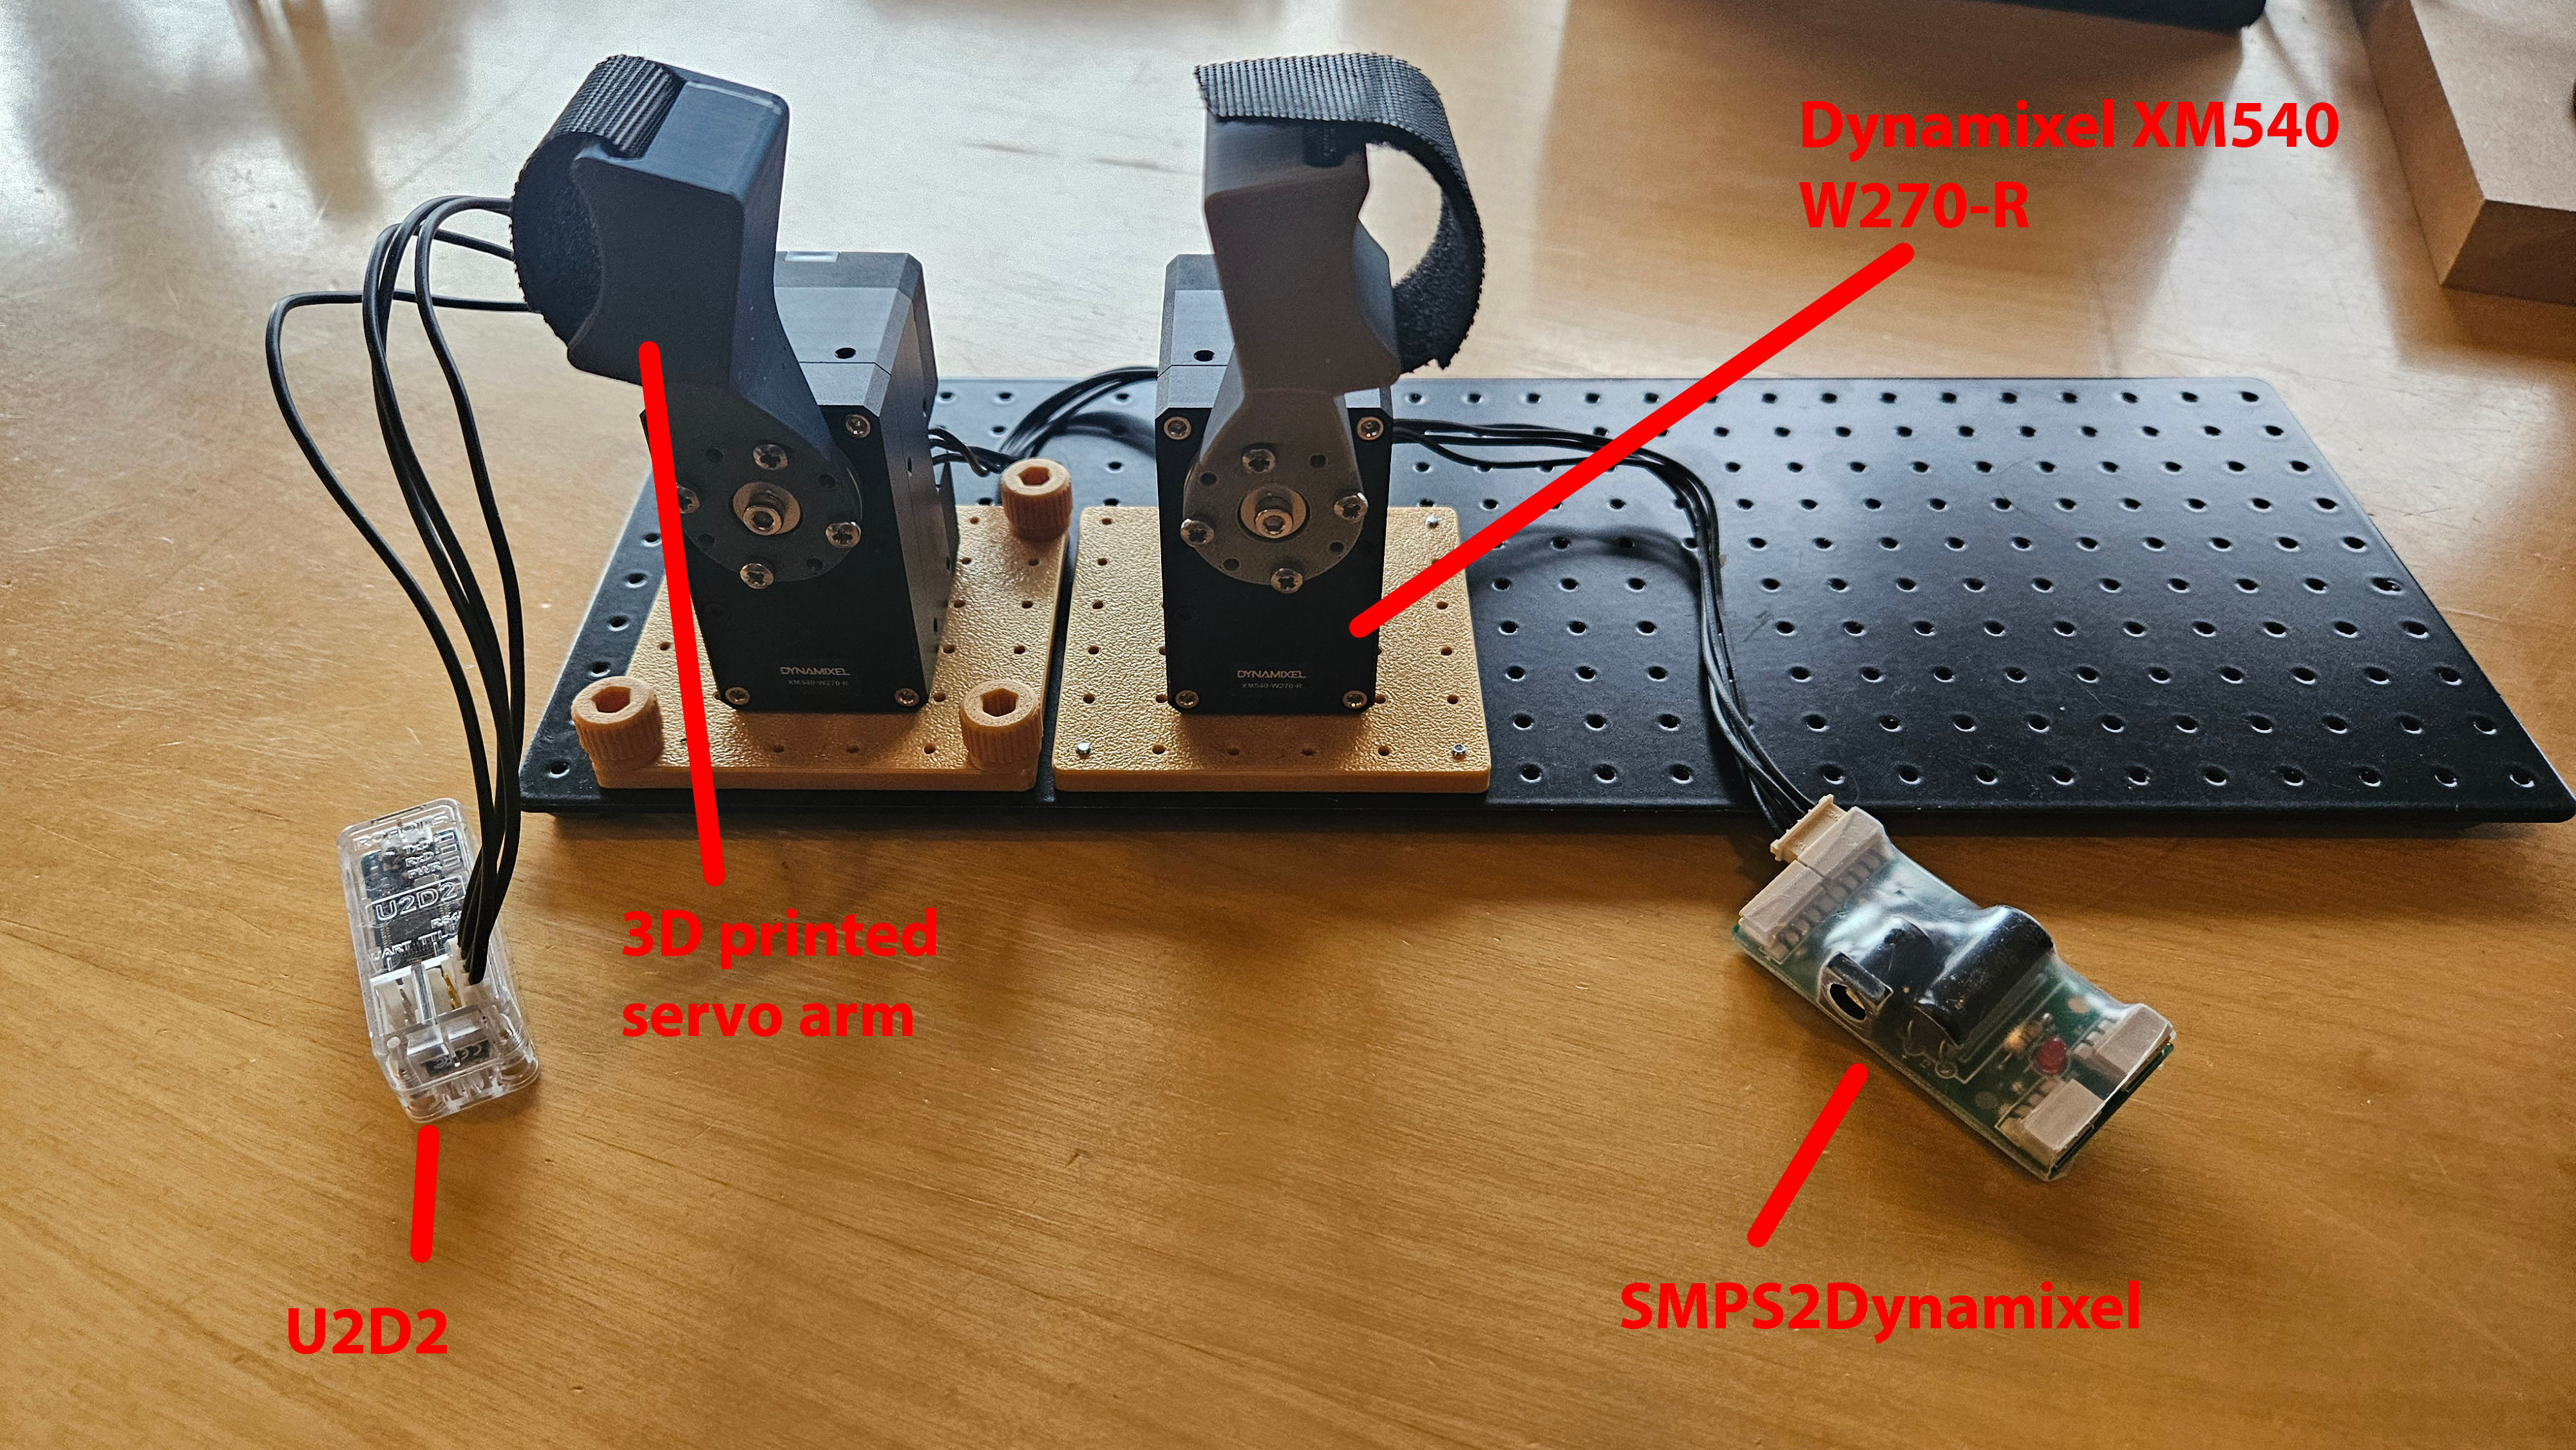
\includegraphics[width=\linewidth]{chapters/exoskeleton/images/background/prototype 1.png}
\caption{Design of \nameone}
\label{fig:design_prototype_one}
\end{figure}

\bigskip \noindent
This design is not a final design, as it is not in the glove form, it can not be worn, and it does not have sensors for global position tracking.